\documentclass[sigconf, review=false, nonacm]{acmart} 
\setlength{\parindent}{0pt} % fix paragraph indentation

% grafos y tablas
\usepackage{tikz}
\usetikzlibrary{shapes.geometric, arrows.meta, positioning}
\tikzstyle{process} = [rectangle, text centered, draw=black]
\tikzstyle{arrow} = [thick, ->, >=stealth]

\usepackage{caption}  % Para personalizar las captions
% Redefinir el formato de las captions para que el texto no sea en negrita
\captionsetup[figure]{labelfont=bf,textfont=normalfont}

\begin{document}

% Metadata del documento
\title{Análisis difuso para el cáculo de sentimientos de publicaciones en redes sociales} \subtitle{Basado en
	el árticulo de Srishti V. \& Seba S. (2019).}

%------------------------- -        Autores        - -------------------------
\author{Elias Sebastián Gill Quintana}
\affiliation{
	\institution{Facultad Politécnica}
	\city{Asunciòn}
	\country{Paraguay}
}
\email{eliasgill42@gmail.com}
\acmYear{2024}

\author{Marcos Raul Flores Duarte}
\affiliation{
	\institution{Facultad Politécnica}
	\city{Asunciòn}
	\country{Paraguay}
}
\email{marcosrflores737@gmail.com}


%---------------------------- -        Preambulo         - ----------------------------
\keywords{Logica Difusa, Social Media, Analisis de Sentimiento.}
\begin{abstract}
	En las redes sociales, comprender el tono emocional de las publicaciones juega un papel crucial para
	analizar el sentimiento de los usuarios y diseñar estrategias efectivas de interacción. Dado que el
	sentimiento puede representarse como una variable gradual con estados lingüísticos utilizando conjuntos
	difusos, este trabajo analiza el sistema propuesto por los autores Srishti V. \& Seba S. \cite{paper}, que
	demuestra un mejor desempeño frente a los sistemas tradicionales de clasificación de sentimientos.\\

	En este trabajo, se estudia un algoritmo propuesto en dicho artículo, el cual consta de seis módulos
	(extracción de datos, preprocesamiento, cálculo de puntaje de sentimiento, sistema de inferencia difusa,
	defusificador y benchmarks) para analizar el sentimiento de publicaciones en redes sociales. Inicialmente, las
	publicaciones son procesadas para extraer características textuales, las cuales se utilizan para calcular
	puntajes de sentimiento basados en patrones lingüísticos. Estos puntajes, junto con reglas predefinidas,
	se introducen en un sistema de inferencia difusa de tipo Mamdani que evalúa el sentimiento, proporcionando
	posibles resultados como negativo, neutral y positivo.\\

	Se comprobó que el sistema propuesto es capaz de analizar tweets de manera rápida y eficiente, manejando
	la incertidumbre del lenguaje natural mediante lógica difusa. Además, demostró ser adecuado para
	aplicaciones en tiempo real, brindando resultados precisos y consistentes en entornos dinámicos.
\end{abstract}

% Genera el título automáticamente
\maketitle

%------------------------------- -        Introduccion         - -------------------------------
\section{Introducción}
Hoy en día, con la masiva adopción de redes sociales, se genera un flujo constante de contenido que refleja
opiniones, emociones y perspectivas de millones de usuarios en tiempo real. Analizar el sentimiento de estos
posts se ha vuelto una herramienta clave para comprender la percepción pública, identificar tendencias y tomar
decisiones estratégicas basadas en datos.\\

Este análisis se realiza utilizando técnicas de procesamiento de lenguaje natural y sistemas de inferencia
que, en algunos casos, integran conjuntos difusos para interpretar la ambigüedad y subjetividad del lenguaje
humano. Estas técnicas permiten clasificar los sentimientos expresados en categorías como positivos, negativos
o neutros, asignándoles una intensidad o grado de pertenencia.\\

Como resultado, se obtienen métricas detalladas sobre la actitud general de los usuarios hacia productos,
marcas o eventos específicos. Esto no solo ayuda a optimizar estrategias de marketing y comunicación, sino
también a mejorar la experiencia del usuario, detectar crisis potenciales en tiempo real y aumentar el
compromiso mediante contenido más relevante y personalizado.

%-------------------- -  Preliminares    - --------------------
\section{Preliminares}
Las operaciones básicas de la matemática incluyen la sumatoria $ \sum $, la multiplicación $ a \times b $
y la división $ \frac{a}{b} $. Entre las operaciones básicas con vectores se encuentran la multiplicación de
vectores $ A \times B $ y el módulo de un vector $ \| A \| $. En el ámbito de la lógica difusa, las
operaciones fundamentales incluyen el operador máximo $ \vee $ y el operador mínimo $ \wedge $.\\

Este artículo se enfoca en la lógica difusa y en los sistemas de control difuso. La lógica difusa extiende los
conjuntos clásicos al agregar una función de pertenencia, que se define como un número real en el intervalo $
	[0, 1] $. Las funciones de pertenencia representan el grado en que un elemento pertenece a un subconjunto
definido por una etiqueta.\\

Los subconjuntos difusos pueden ser operados mediante determinados operadores, y también es posible realizar
operaciones entre ellos. Al aplicar un operador a un solo conjunto, se obtiene otro conjunto; lo mismo ocurre
cuando se realiza una operación entre conjuntos. \\

En un sistema de control difuso, siempre se realiza un proceso de fusificación, el cual ocurre de forma
continua y actúa como la puerta de entrada al sistema de inferencia difusa. Este procedimiento matemático
convierte un elemento del universo de discurso (como una variable o medida del proceso) en un valor dentro de
las funciones de membresía a las cuales pertenece.\\

Los controladores difusos operan mediante reglas que combinan uno o más conjuntos borrosos de entrada
(denominados antecedentes o premisas) y asignan un conjunto borroso de salida (denominado consecuente o
consecuencia). Estas reglas implican conjuntos difusos, lógica difusa e inferencia difusa, y se conocen como
``reglas borrosas'' o ``fuzzy rules''. Las reglas tienen la estructura SI-ENTONCES.\\

Las reglas difusas de Mamdani se componen de dos partes: un antecedente y un consecuente. A estas reglas se
les aplican los operadores difusos máximo y mínimo para obtener un conjunto difuso de salida, el cual, junto
con las salidas de otras reglas, constituye la salida final del sistema.\\

Finalmente, el sistema de inferencia difusa obtiene una conclusión a partir de la información de entrada, pero
dicha conclusion se encuentra en términos de un conjunto ``borroso``. El proceso de defusificación
(\textit{defusification}) consiste en convertir este conjunto difuso en un número real que represente
adecuadamente los resultados de la etapa de agregacion, de modo que este resultado es interpretable por
nuestros modelos. Por esta razón existen diferentes métodos de defusificación, cada uno de los cuales arroja
resultados distintos.

%------------------------------        Arquitectura del sistema         ------------------------------
\section{Arquitectura del Sistema}

El sistema de recomendación difuso propuesto contiene 6 módulos, los cuales seran listados a continuacion:
\begin{enumerate}
	\item \textbf{Lector de datasets}: La etapa inicial en el análisis de sentimientos consiste en la lectura
	      y procesamiento del conjunto de datos. En este caso, se utiliza un dataset de sentimientos extraídos
	      de tweets, el cual está estructurado específicamente para facilitar el análisis de emociones y
	      opiniones. Este debe contener, como mínimo, dos columnas clave: el texto de los tweets y una etiqueta
	      que indique el sentimiento asociado.

	\item \textbf{Lexicón de Sentimientos}: Para determinar la polaridad inicial de los sentimientos
	      expresados en los tweets, se emplea el lexicón de sentimientos VADER (Valence Aware Dictionary and
	      Sentiment Reasoner). Esta etapa genera una puntuación numérica que sirve como base para la posterior
	      fusificación.

	\item \textbf{fusificación}: En un sistema basado en lógica difusa, el primer paso es la fusificación.
	      Este proceso convierte valores numéricos a conjuntos difusos. En el análisis de sentimientos, este
	      paso se aplica a los resultados cuantitativos obtenidos a partir del lexicón VADER.

	\item \textbf{Sistema de Inferencia}: Este módulo implementa un sistema de reglas difusas diseñado
	      para inferir el sentimiento general basándose en los puntajes de sentimiento positivo y negativo
	      obtenidos tras la fusificación. Estas reglas utilizan un conjunto predefinido que relaciona las
	      entradas difusas con una salida difusa que clasifica el sentimiento en categorías como Positivo,
	      Negativo y Neutral.

	\item \textbf{Defusificador}: Finalmente, la salida difusa generada por el sistema de inferencia se
	      transforma en un valor discreto a través del proceso de defusificación, permitiendo así un análisis
	      más claro y directo de los resultados obtenidos.

	\item \textbf{Benchmarks}: Para evaluar el rendimiento del sistema de recomendación difuso, se utilizan
	      distintas metricas en base al tiempo de ejecucion y la precision del resultado.
\end{enumerate}

% Imagen de el sistema propuesto
\begin{figure}[ht]
	\centering
	\resizebox{\linewidth}{!}{ % Ajusta el tamaño al ancho de la página
		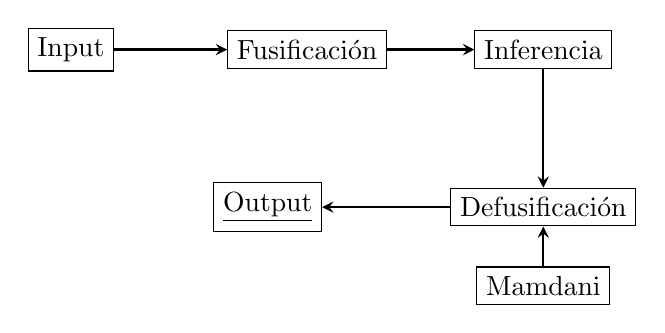
\begin{tikzpicture}[node distance=2cm]
			% Nodes
			\node (input) [process] {Input};
			\node (fuzz) [process, right of=input, xshift=1cm] {Fusificación};
			\node (compute) [process, right of=fuzz, xshift=1cm] {Inferencia};
			\node (defuzz) [process, below of=compute, yshift=0cm] {Defusificación};
			\node (mamdani) [process, below of=defuzz, yshift=1cm] {Mamdani};
			\node (aggregate) [process, left of=defuzz, xshift=-1.5cm] {\underline{Output}};
			% Arrows
			\draw [arrow] (input.east) -- (fuzz.west);
			\draw [arrow] (fuzz.east) -- (compute.west);
			\draw [arrow] (compute.south) -- (defuzz.north);
			\draw [arrow] (defuzz.west) -- (aggregate.east);
			\draw [arrow] (mamdani.north) -- (defuzz.south);
		\end{tikzpicture}
	}
	\caption{Diagrama de flujo del sistema.}
	\label{fig:flow-diagram}
\end{figure}

%-------------------------------        Metodologia        -------------------------------
\section{Metodologia}
\subsection{Lector de datasets}
Un dataset, o conjunto de datos, es una colección organizada de información que se estructura en filas y
columnas. Para este sistema utilizamos los siguientes datasets:
\begin{itemize}
	\item \href{https://www.kaggle.com/datasets/krishbaisoya/tweets-sentiment-analysis}{Sentiment140-test}
	\item
	      \href{https://www.kaggle.com/datasets/azzouza2018/semevaldatadets?resource=download&select=semeval-2013-test.csv}{SemEval2013-test}
	\item
	      \href{https://www.kaggle.com/datasets/azzouza2018/semevaldatadets?resource=download&select=semeval-2017-test.csv}{SemEval2017-test}
\end{itemize}

Una vez cargado en memoria, debemos realizar la limpieza de los datos, siendo este un paso crítico para
garantizar resultados precisos en las etapas posteriores, reduciendo el ruido en los datos de prueba y
mejorando la precision en las etapas de análisis lexicográfico y fusificación.\\

Primeramente se realiza la eliminación de caracteres especiales (como puntos comas, asteriscos, numeros, etc),
menciones (como "@usuario"), hashtags y URLs. Del mismo modo, se realiza la normalización del texto,
transformando palabras abreviadas o contraídas a sus formas completas, como por ejemplo: ``won't'' a ``will
not'' o ``can't'' a ``cannot''.

\subsection{Lexicón de Sentimientos}
Para identificar la polaridad inicial del sentimiento en los tweets,
se utiliza el lexicón de sentimientos de VADER (Valence Aware Dictionary and sentiment Reasoner).
Este modelo es ampliamente utilizado debido a su capacidad para manejar datos informales como los tweets.
El lexicón de VADER asigna puntuaciones de sentimiento a palabras individuales y frases, lo que permite calcular
tres métricas clave para cada tweet:

\begin{enumerate}
	\item \textbf{Negativa:} Representa la proporción del texto con carga emocional negativa.
	\item \textbf{Neutral:} Indica la proporción de contenido emocionalmente neutro.
	\item \textbf{Positiva:} Define el nivel de contenido emocional positivo en el texto.
\end{enumerate}

La salida de esta etapa proporciona un punto de partida cuantitativo para la fusificación.

\subsection{Fusificación}
La fusificación es el paso inicial en un sistema de lógica difusa y su propósito es el de traducir valores
numéricos exactos en grados de pertenencia difusos. La fusificación se aplica a las métricas de sentimiento
obtenidas del lexicón VADER, métricas que luego se convierten en conjuntos difusos que representan la intensidad
de los sentimientos negativos, neutros y positivos en cada tweet.\\

Para realizar la fusificación utilizaremos la función de membresía triangular. Esta
función se caracteriza por tener un pico en el valor medio y una pendiente lineal en ambos lados. Este tipo de
funciones se definen con tres parámetros clave:

\begin{enumerate}
	\item El límite izquierdo donde la pertenencia comienza a ser mayor que cero.
	\item El valor pico, donde la pertenencia es máxima.
	\item El límite derecho donde la pertenencia vuelve a cero.
\end{enumerate}

En esta etapa, las puntuaciones negativa, neutral y positiva obtenidas, son convertidas en valores difusos
utilizando funciones de membresía triangulares. Este enfoque es elegido por su simplicidad y capacidad para
modelar la incertidumbre inherente en los datos lingüísticos.
$$
	\mu(x) =
	\begin{cases}
		0,                   & \text{si } x \leq a \text{ o } x \geq c, \\
		\frac{x - a}{b - a}, & \text{si } a \leq x < b,                 \\
		\frac{c - x}{c - b}, & \text{si } b \leq x < c.
	\end{cases}
$$
Cada una de las métricas negativa, neutral y positiva es transformada en conjuntos difusos con valores
entre 0 y 1, donde:

- Baja: Representa valores bajos de pertenencia para una métrica.

- Media: Indica valores intermedios de pertenencia.

- Alta: Denota niveles altos de pertenencia.

Por ejemplo, si un tweet tiene una puntuación positiva de 0.7 según el lexicon de Vader,
su valor difuso podría ser calculado como perteneciente parcialmente a los conjuntos Media y Alta,
con grados de pertenencia determinados por las funciones triangulares.

\subsection{Sistema de inferencia}
Este módulo implementa un sistema de reglas difusas diseñado para inferir el sentimiento general de un
tweet basándose en los puntajes de sentimiento positivo y negativo obtenidos tras la fusificación.
El sistema se fundamenta en un conjunto predefinido de reglas difusas que relacionan las entradas
difusas (nivel de positividad y negatividad) con una salida difusa (clasificación del sentimiento).

\subsubsection{Implementación}
El sistema de reglas difusas utiliza las siguientes reglas basadas en la lógica difusa Mamdani:
\begin{itemize}
	\item \textbf{Regla 1}: Si el nivel de positividad es bajo y el nivel de negatividad es bajo, entonces el
	      sentimiento es neutral.
	\item \textbf{Regla 2}: Si el nivel de positividad es medio y el nivel de negatividad es bajo, entonces el
	      sentimiento es positivo.
	\item \textbf{Regla 3}: Si el nivel de positividad es alto y el nivel de negatividad es bajo, entonces el
	      sentimiento es positivo.
	\item \textbf{Regla 4}: Si el nivel de positividad es bajo y el nivel de negatividad es medio, entonces el
	      sentimiento es negativo.
	\item \textbf{Regla 5}: Si el nivel de positividad es medio y el nivel de negatividad es medio, entonces
	      el sentimiento es neutral.
	\item \textbf{Regla 6}: Si el nivel de positividad es alto y el nivel de negatividad es medio, entonces el
	      sentimiento es positivo.
	\item \textbf{Regla 7}: Si el nivel de positividad es bajo y el nivel de negatividad es alto, entonces el
	      sentimiento es negativo.
	\item \textbf{Regla 8}: Si el nivel de positividad es medio y el nivel de negatividad es alto, entonces el
	      sentimiento es negativo.
	\item \textbf{Regla 9}: Si el nivel de positividad es alto y el nivel de negatividad es alto, entonces el
	      sentimiento es neutral.
\end{itemize}

A continuación, se presenta una tabla que resume las reglas difusas implementadas en el sistema:

\begin{table}[h!]
	\centering
	\begin{tabular}{|c|c|c|c|}
		\hline
		\textbf{Regla} & \textbf{Nivel de Positividad} & \textbf{Nivel de Negatividad} & \textbf{Resultado} \\ \hline
		1              & Bajo                          & Bajo                          & Neutral            \\ \hline
		2              & Medio                         & Bajo                          & Positivo           \\ \hline
		3              & Alto                          & Bajo                          & Positivo           \\ \hline
		4              & Bajo                          & Medio                         & Negativo           \\ \hline
		5              & Medio                         & Medio                         & Neutral            \\ \hline
		6              & Alto                          & Medio                         & Positivo           \\ \hline
		7              & Bajo                          & Alto                          & Negativo           \\ \hline
		8              & Medio                         & Alto                          & Negativo           \\ \hline
		9              & Alto                          & Alto                          & Neutral            \\ \hline
	\end{tabular}
	\caption{Reglas difusas definidas en el sistema.}
	\label{table:reglas_difusas}
\end{table}

\subsection{Defusificador}
La defusificación es el procedimiento mediante el cual las salidas difusas del sistema de inferencia se
convierten en un valor numérico específico. Este valor es utilizado para determinar la clasificación final del
sentimiento del tweet en una de las siguientes categorías: positivo, negativo o neutral.

Para este módulo, se emplea el método del centroide, una técnica ampliamente utilizada que consiste en hallar
el "centro de gravedad" o "punto promedio" del área bajo la curva del conjunto difuso. El mismo esta dado
formula:
$$
	C = \frac{\int_{\text{dom}(x)} x \cdot \mu(x) \, dx}{\int_{\text{dom}(x)} \mu(x) \, dx}
$$

\subsection{Benchmarks}
Para medir el desempeño del sistema, se analizaron métricas relacionadas
con el tiempo de ejecución y la precisión obtenida en los datasets empleados.
Asimismo, se realizaron comparaciones de los resultados entre los diferentes conjuntos de datos,
cuyos detalles se presentan en la sección de resultados.

%-------------------------------        Resultados         -------------------------------
\section{Resultados}
En esta seccion se muestran los resultados de la mediciones tomadas del rendimiento del modelo sobre los 3
datasets escogidos. Primeramente se preseta un grafico de barras el cual representa los valores de
pertenencia de sentimiento calculados en la etapa de fusificacion. Posteriormente un grafico de dispersión que
representa las coincidencias de los sentimientos calculados con los datos esperados y por ultimo las metricas
de precision y tiempo de ejecucion para los distintos datasets.

\subsection{Valores de pertenencia}
A continuación, se presentan los resultados de los puntajes de sentimiento para los primeros
40 tweets de cada dataset.

\begin{figure}[H]
	\centering
	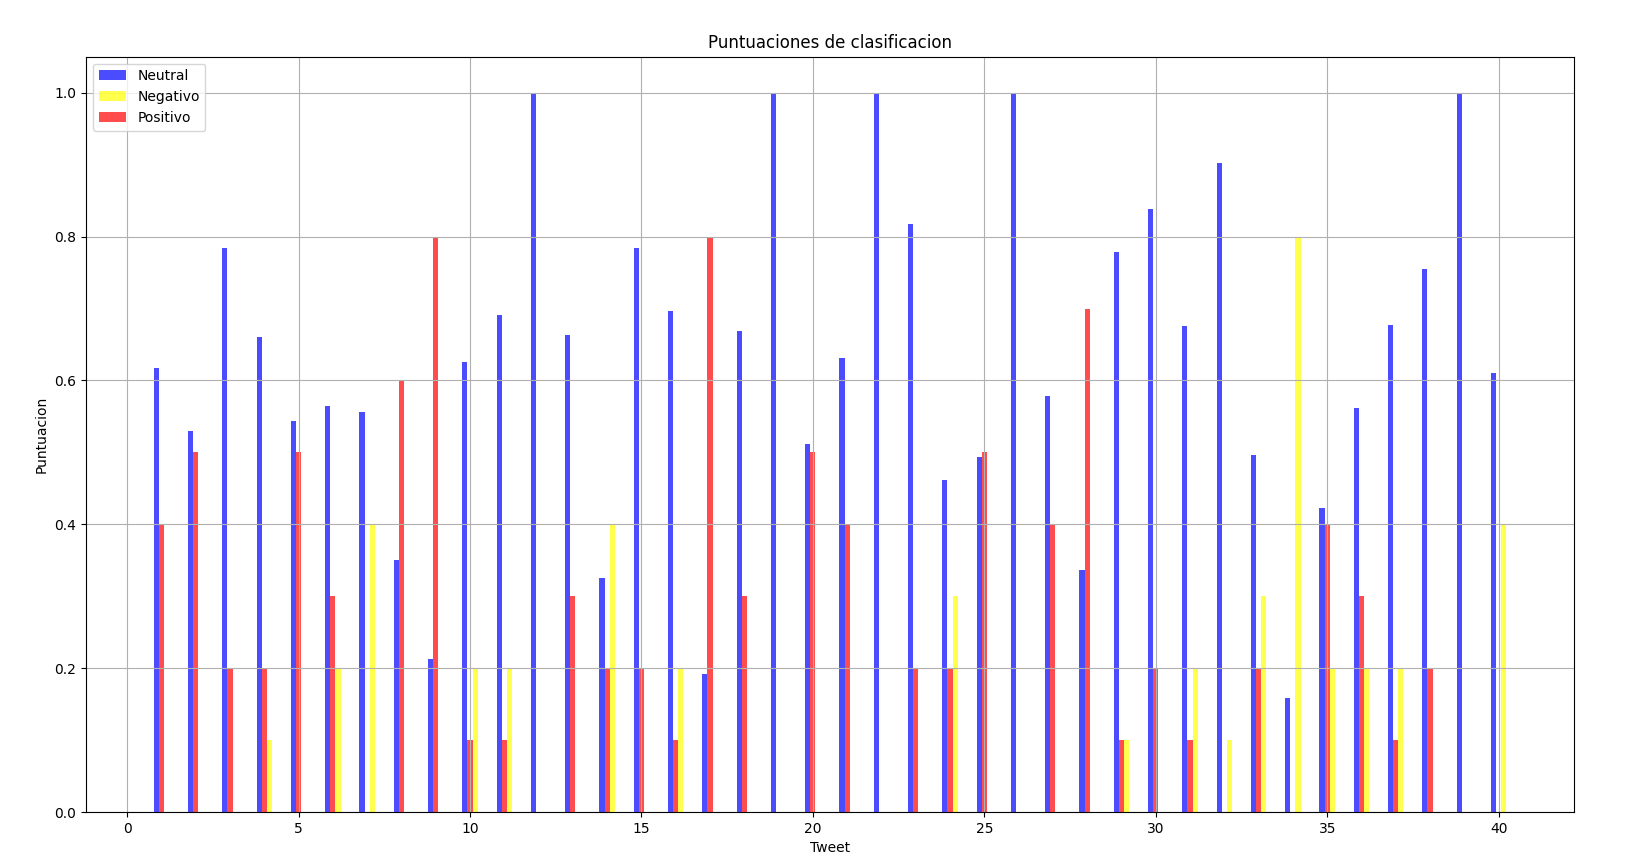
\includegraphics[width=\linewidth]{../results/barras/sentiment140.png}
	\caption{Resultados de interpretación del sentimiento para el dataset Sentiment140-test.}
	\label{fig:sentiment140}
\end{figure}

\begin{figure}[H]
	\centering
	\includegraphics[width=\linewidth]{../results/barras/semeval2013.png}
	\caption{Resultados de interpretación del sentimiento para el dataset SemEval2013-test.}
	\label{fig:semeval2013}
\end{figure}

\begin{figure}[H]
	\centering
	\includegraphics[width=\linewidth]{../results/barras/semeval2017.png}
	\caption{Resultados de interpretación del sentimiento para el dataset SemEval2017-test.}
	\label{fig:semeval2017}
\end{figure}

% -- Dispersion --
\subsection{Gráficos de Dispersión}
A continuación una comparativa de los resultados obtenidos en los tres datasets, mostrando la dispersión de los
puntajes de sentimiento calculado en cada uno de ellos con respecto al sentimiento esperado.

\begin{figure}[H]
	\centering
	\includegraphics[width=0.45\textwidth]{../results/dispersion/semeval2013.png}
	\caption{SemEval2013}
	\label{fig:semeval2013}
\end{figure}

La Figura \ref{fig:semeval2013} muestra la dispersión de los puntajes de sentimiento calculados para el dataset SemEval2013.
Se observa una diferencia notable entre los valores esperados y obtenidos, con porcentaje de 45 porciento de precisión.

\begin{figure}[H]
	\centering
	\includegraphics[width=0.45\textwidth]{../results/dispersion/semeval2017.png}
	\caption{SemEval2017}
	\label{fig:semeval2017}
\end{figure}

La Figura \ref{fig:semeval2017} muestra la dispersión de los puntajes de sentimiento calculados para el dataset SemEval2017.
Se observa un resultado basntane similar que con SemEval2013.

\begin{figure}[H]
	\centering
	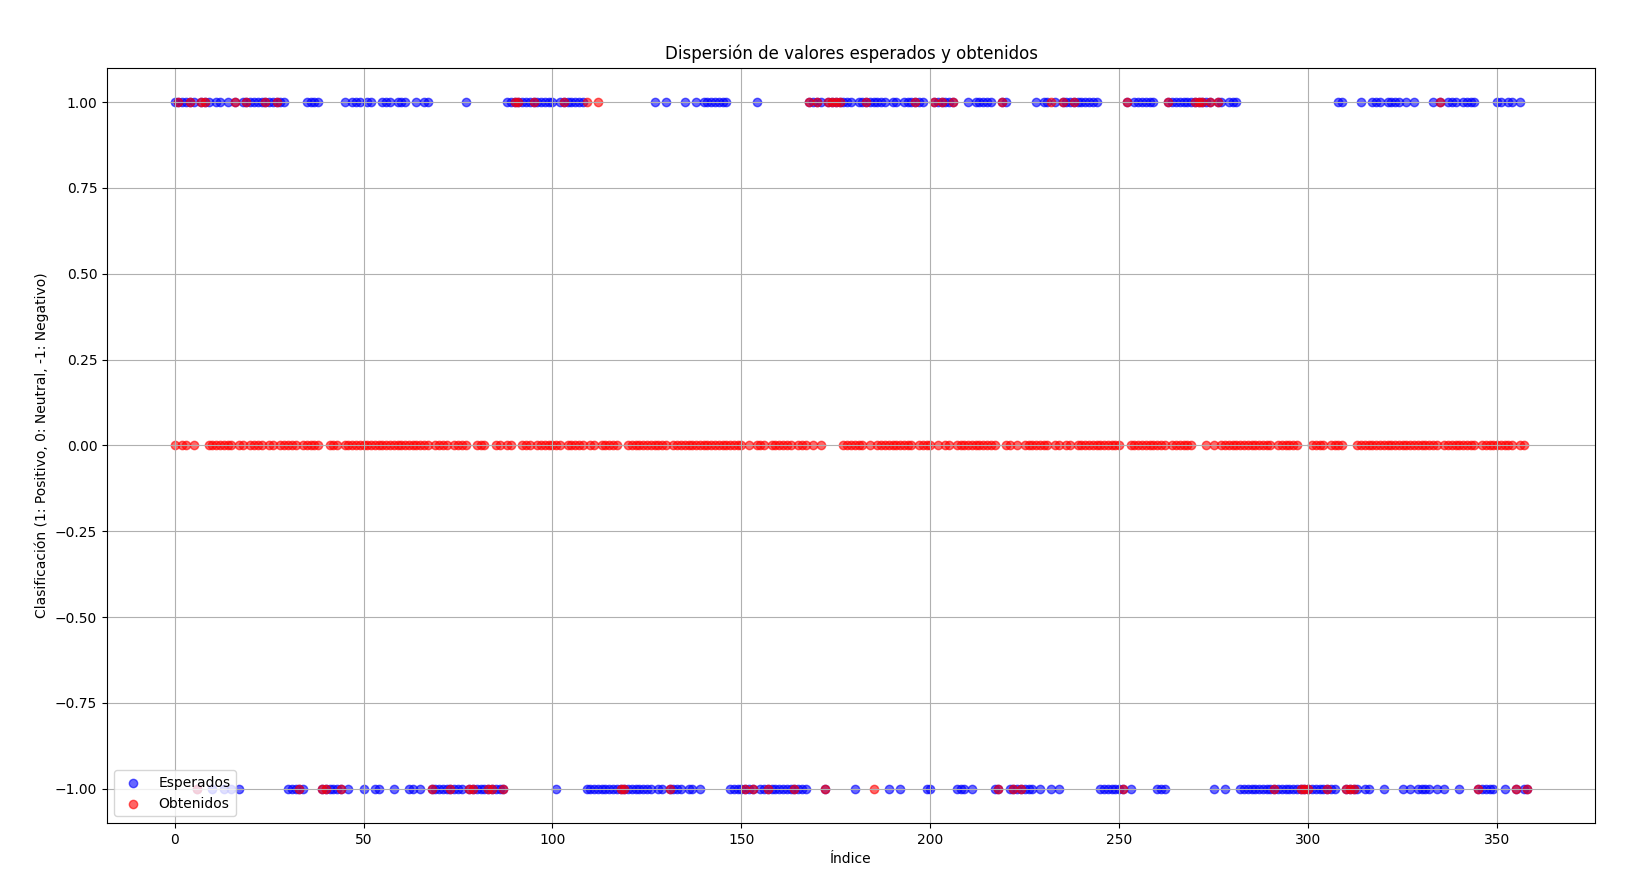
\includegraphics[width=0.45\textwidth]{../results/dispersion/sentiment140.png}
	\caption{sentiment140}
	\label{fig:sentiment140}
\end{figure}

La Figura \ref{fig:sentiment140} ilustra la dispersión de los puntajes de sentimiento para el dataset Sentiment140.
Se puede apreciar una dispersión mayor, lo que sugiere que el sistema estaría teniendo
dificultades para interpretar correctamente los sentimientos en este dataset.

%-------------------------------        Análisis         -------------------------------
\subsection{Análisis del tiempo de ejecución}
El análisis del tiempo de ejecución es crucial para evaluar la eficiencia del sistema
de análisis de sentimientos propuesto. A continuación, se presentan los resultados obtenidos
para cada uno de los datasets utilizados:

\begin{itemize}
	\item \textbf{SemEval2017}: Este dataset contiene un total de 11,977 tweets. El tiempo total
	      de ejecución fue de 7.2 segundos, lo que resulta en un tiempo promedio por tweet de
	      aproximadamente 0.000601 segundos. La precisión obtenida fue del 52\%.

	\item \textbf{SemEval2013}: Con un total de 3,545 tweets, el tiempo total de ejecución para este
	      dataset fue de 2.302 segundos. Esto se traduce en un tiempo promedio por tweet de
	      aproximadamente 0.000649 segundos. La precisión obtenida fue del 45\%.

	\item \textbf{Sentiment140}: Este dataset contiene 359 tweets. El tiempo total de ejecución
	      fue de 0.221 segundos, resultando en un tiempo promedio por tweet de aproximadamente 0.000617 segundos.
	      a precisión obtenida fue del 19\%.
\end{itemize}

En general, el tiempo de ejecución promedio por tweet se mantuvo en un rango muy eficiente, con valores que oscilan entre 0.000601 y 0.000649 segundos. Esto demuestra que el sistema es capaz de procesar grandes volúmenes de datos en un tiempo razonable, lo cual es esencial para aplicaciones en tiempo real.

%-------------------------------        Conclusion         -------------------------------
\section{Conclusión}
En conclusión, el sistema de análisis de sentimientos basado en lógica difusa propuesto en este trabajo ha
demostrado ser una herramienta efectiva para calcular correctamente el tono emocional de publicaciones en
redes sociales. Mediante la implementación de un sistema de inferencia difusa, se ha logrado manejar la
incertidumbre y ambigüedad del lenguaje natural, proporcionando resultados con una precisión de hasta el
52\%.\\

Este enfoque permite analizar el sentimiento con una precision aceptable y con una enorme rapidez. Si bien los
resultados son prometedores, aún hay margen de mejora en el sistema de inferencia a fin de lograr una mayor
precisión en el análisis de sentimientos.\\

En general, este trabajo demuestra el potencial del análisis de sentimientos basado en lógica difusa para
comprender mejor las emociones expresadas en contenido generado por usuarios en redes sociales.

% Bibliografía
\nocite{libro, libro2}
\bibliographystyle{ACM-Reference-Format}
\bibliography{bibliography}

\end{document}
